\documentclass[a4paper, 10pt]{article}
\usepackage[utf8]{inputenc}
\usepackage[T1]{fontenc}
\usepackage{ngerman, lmodern}
%\usepackage[left=3cm, right=3cm]{geometry}

\newcommand{\mytitle}{Untersuchung und Kontrolle von chaotischem Verhalten am Doppelpendel}
\newcommand{\myauthor}{Jann Horn und Hannes Riechert}

\usepackage{graphicx, wrapfig, subfigure, color, amsmath, amsthm}
\usepackage{fancyhdr}
  \lhead{\myauthor}
  \chead{}
  \rhead{\nouppercase\leftmark}
  \lfoot{}
  \cfoot{\thepage}
  \rfoot{}

\usepackage[numbers]{natbib}
\usepackage{setspace}
  \onehalfspacing % Zeilenabstand
% \usepackage[numbers]{natbib} % bibliography

\newcommand{\TODO}{\textcolor{red}{ \textbf TODO }}
\newcommand{\mathematik}{\begin{equation*}\begin{aligned}}
\newcommand{\mathematikstop}{\end{aligned}\end{equation*}}
\renewcommand{\phi}{\varphi} % make "stroked" phi look "loopy"
\renewcommand{\rho}{\varrho}
\newcommand{\half}{\frac{1}{2}} % 1/2
\newcommand{\phid}{\dot{\phi}}  % phi with one dot
\newcommand{\intend}{\,\mathrm{d}} % end of integral
\newcommand{\EQU}{\qquad\bigg|\,} % separator for explanations for equivalent rearrangements

\clubpenalty = 10000
\widowpenalty = 10000
\displaywidowpenalty = 10000

\title{\mytitle}
\author{\myauthor}
%\date{ }

\begin{document}
\maketitle
\begin{abstract}
In unserem Projekt beschäftigen wir uns mit dem Verhalten von chaotischen Doppelpendeln. Wir wollen aus der aktuellen Bewegung eines Doppelpendels den weiteren Bewegungsablauf in einem kurzen Zeitintervall extrapolieren und dann versuchen, diese Bewegung zu beeinflussen.

Hierzu wollen wir zunächst ein Doppelpendel konstruieren, bei dem Daten über den aktuellen Bewegungszustand erfasst werden können. Diese Daten sollen in Echtzeit von einem Computer ausgewertet werden, um laufend eine Prognose an die Messwerte anzupassen. Anhand dieser Prognose soll dann entschieden werden, ob das Pendel eine unerwünschte Bewegung durchführen wird, und wenn nötig, soll mithilfe mehrerer Spulen eine korrigierende magnetische Kraft erzeugt werden. Es könnte zum Beispiel erwünscht sein, einen Überschlag zu vermeiden.
\end{abstract}

\newpage
\pagestyle{fancy}
\tableofcontents

\newpage

\section{Einleitung}
Als erstes haben wir an den mathematisch genauen Schwingungsdifferenzialgleichungen für das Doppelpendel gearbeitet.
Und eine vollkommen theoretische Simulation von einem Doppelpendel realisiert.

Erst danach haben wir mit der Konstruktion des Modells, das in Abbildung (\TODO ref) zu sehen ist begonnen.

\section{Simulation}

\subsection{Mathematischer Hintergrund}

Der Lösungsansatz über die Euler"=Lagrange Gleichung ist von der englischen Wikipedia übernommen worden.
\citep{wikidoublependulum}

Die Gleichungen wurden nur um die Konstanten $k_1$ bis $k_5$ erweitert, um sie an unser Pendel anpassen zu können, das keine gleichmäßige Massenverteilung aufweist.

(\TODO wo ist die vollständige Herleitung?)

Die Position der Pendelarme kann durch die zwei generalisierten Koordinaten $\phi_1$ und $\phi_2$ beschrieben werden, die die Winkel der Arme angeben.
Alle Winkel werden relativ zu senkrechten angegeben, also bedeutet $0^\circ$ senkrecht nach unten und zum Beispiel $45^\circ$ nach unten rechts.
Für die vollständige Angabe des Zustands des Systems ist zusätzlich noch der generalisierte Impuls hier als $p_1$ und $p_2$ bezeichnet, vonnöten.

Aus den Funktionen $\dot{p}_1$, $\dot{p}_2$, $\phid_1$ und $\phid_2$ setzt sich das System von Differentialgleichungen zusammen, mit denen aus dem aktuellen Zustand der Zustand des Systems zu jeder gegebenen Zeit berechnen lässt.
Die Berechnung kann zum Beispiel Iterativ mit dem Runge"=Kutta"=Verfahren erfolgen.

\begin{figure}[bht]
  \includegraphics[width=\textwidth]{charts/mathsketch_dia.png}
  \caption{Zeichnung der Pendelarme zur Bedeutung der Längenangaben}
  \label{fig:mathsketch}
\end{figure}

In der Abbildung \ref{fig:mathsketch} ist zu erkennen, wie die Längenangaben zu interpretieren sind.
An der ersten Achse ist das Doppelpendel aufgehängt.
$l_{1a}$ ist eine negative Zahl und gibt an, wie lang das erste Pendel auf der Seite ist, an der nicht das zweite Pendel hängt.
$l_1$ gibt den Abstand der beiden Achsen an und $l_{1b}$ beschreibt als positive Zahl die Länge des ersten Pendels in Richtung des zweiten Pendels.
$l_{2a}$ und $l_{2b}$ geben die beiden Längen des zweiten Pendelarms an relativ zu seiner Achse.

Diese Längenangaben sind in den Konstanten $k_1$ bis $k_5$ wiederzufinden, die darauf abziehlen die Eigenschaften des Pendels so genau wie möglich beschreiben zu können, indem zwei Dichtefunktionen $\rho(r)$ über den Abstand $r$ von der jeweiligen Achse für die beiden Pendelarme angegeben werden.

(\TODO soll das hier wirklich stehen:) Diese Konstanten sind nicht dazu gedacht, dass sie ausgemessen werden, sondern unsere Vorstellung war später unse Gleichungen damit zu kalibrieren.

Die Differentialgleichungen lauten wie folgt:
\mathematik
\phid_1 &= \frac{k_4 p_1 - k_5 l_1 p_2 cos(\phi_1 - \phi_2)}{k_1 k_4 + l_1 \cdot (k_3 k_4 - k_5^2 l_1 cos^2(\phi_1 - \phi_2))} \\[0.5\baselineskip]
\phid_2 &= \frac{k_1 p_2 + l1 \cdot (k_3 p_2 - k_5 p_1 cos(\phi_1 - \phi_2))}{k_1 k_4 + l_1 \cdot (k_3 k_4 - k_5^2 l_1 cos^2(\phi_1 - \phi_2))} \\[0.5\baselineskip]
\dot{p}_1 &= -l_1 \phid_1 \phid_2 k_5 sin(\phi_1 - \phi_2) - g k_2 sin \phi_1 - g l_1 k_3 sin \phi_1 \\[0.5\baselineskip]
\dot{p}_2 &= l_1 \phid_1 \phid_2 k_5 sin(\phi_1 - \phi_2) - g k_5 sin \phi_2 \\[0.5\baselineskip]
\mathematikstop
Und die Konstaten $k_1$ bis $k_5$ sind so definiert:
\mathematik
k_1 &= \int^{l_{1b}}_{l_{1a}} \rho_1(r) \; r^2 \intend r
\qquad && k_2 &= \int^{l_{1b}}_{l_{1a}} \rho_1(r) \; r \intend r \\
k_3 &= \int^{l_{2b}}_{l_{2a}} \rho_2(r) \intend r
&& k_4 &= \int^{l_{2b}}_{l_{2a}} \rho_2(r) \; r^2 \intend r \\
k_5 &= \int^{l_{2b}}_{l_{2a}} \rho_2(r) \; r \intend r \\
\mathematikstop

\subsection{Software}
Wir haben in Haskell eine Simulation geschrieben, die das klassische Runge"=Kutta"=Verfahren anwendet.
\citep{wikirungekutta}

Die Simulation generiert dann eine CSV-Datei, die in regelmäßigen Zeitintervallen die Winkel und die verschiedenen Energien enthält.
Auf die Winkel wird danach die diskrete Fourier"=Transformation mit einem sich bewegenden Fester angewendet, um Perioden in der Bewegung erkenn zu können.
Nachdem die Winkel und ihre Fourier"=Transformation berechnet sind, werden die Daten angezeigt.
In Abbildung \ref{fig:hssim} ist eine Screenshot der Anzeige zu sehen.

\begin{figure}[bht]
  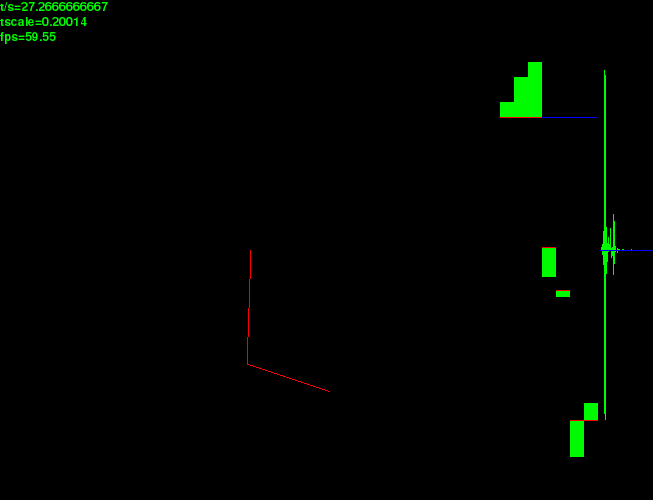
\includegraphics[width=\textwidth]{images/haskell_simulation_fwindow1000_cropped.png}
  \caption{Screenshot der Simulation}
  \label{fig:hssim}
\end{figure}

Zu erkennen ist die aktuelle Position des Pendels als rote Skizze.
Die dicken grünen Balken rechts daneben zeigen auf einer für alle dicken Balken gleichen Skalierung die Energien $T_1$, $T_2$, $T_{Ges}$, $V_1$, $V_2$, $V_{Ges}$ und $E_{Ges}$ in der Reihenfolge von links nach rechts an.
Der blaue Stricht zeigt die Nulllinie an, die roten Striche die Anfangswerte der Energien.
Die potentielle Energie ist Anfangs kleiner null, weil der Koordinatenurspung in der ersten Achse liegt und damit die Schwerpunkte der Pendelarme unterhalb des Bezugspunkts liegen.
Die Gesamtenergie $E_{Ges} = T_{Ges} + V_{Ges}$ sollte bei einer perfekten Simulation nicht von ihrem Anfangswert abweichen. Aber wie zu sehen ist, wächst sie in unserer Simulation stetig.
Dies ist auf die Ungenauigkeiten der numerischen Simulation zurückzuführen.

Rechts neben den dicken Balken ist die diskrete Fourier"=Transformation der Winkel zu sehen.
Oberhalb der blauen Linie wird die Transformation von $\phi_1$ angezeigt, unterhalb die Transformation von $\phi_2$.
Jeder der Balken ist einen Pixel breit und bedeutet eine Frequenz aus dem Ergebnis.
Der Abstand nach rechts vom ersten Balken aus ist proportional zur Frequenz.
Aus dem aktuell zu sehenden Fester ist zum Beispiel für den ersten Pendelarm abzulesen, dass sich das Pendel regelmäßg von rechts nach links bewegt, zu erkennen am rechten Ausschlag, und der zweite Pendelarm eine schwächere aber schnellere Schwingung erzeugt, zu sehen als linker Ausschlag.

Die Transformation des zweiten Pendelarms zeigt eine starke Korrelation mit der Transformation des ersten Pendelarms. Das liegt daran, dass für diese Abbildung eine relativ stark periodische Einstellung des Systems gewählt wurde, und der zweite Pendelarm eine dem ersten Pendelarm ähnliche Bewegung durchführt.


\section{Der Aufbau des Modells}

\begin{figure}
  \includegraphics[width=\textwidth]{charts/pendulumsketch.png}
  \caption{Position der Spulen in Polarkoordinaten}
  \label{fig:pendulumsketch}
\end{figure}

Um das Verhalten des Doppelpendels zu beeinflussen, muss der Zustand des Pendels
erfasst werden können. Zu diesem Zweck verwenden wir einen am Ende des Pendels
befestigten Magneten, der in am Rahmen montierten Spulen elektrische Ströme
hervorruft, wenn er an diesen vorbeibewegt wird.

Diese Ströme verursachen Spannungsschwankungen an den Spulen. Um diese zu messen,
verbinden wir alle Spulen auf einer Seite mit einer 3,3 V--Span"-nungs"-quel"-le und auf der
anderen mit den 16 Analogeingängen eines ATmega2560--Mi"-kro"-con"-trollers. Der auf einen
Messbereich von 0 bis 5V eingestellte Mikrocontroller iteriert dann in einer Endlosschleife
über alle Eingänge, misst die an ihnen momentan anliegenden Spannungen mit einer
Auflösung von 10 Bit und leitet sie an einen Serial--to--USB--Konverter weiter. Der Messbereich
ist dadurch zwar relativ zur Grundspannung asymmetrisch --- der maximale negative Ausschlag beträgt
theoretisch 3,3 V, während der maximale positive Ausschlag $ 5V - 3,3 V = 1.7 V $ beträgt ---, aber
Spannungsregler für 3,3 V sind einfacher verfügbar als welche für 2,5 V.
% zusätzliches argument: negative spitzen machen mist?

Der Serial--to--USB--Konverter ist per USB an einen Computer angeschlossen, der die 5V--Stromversorgung
bereitstellt und die Messwerte aufzeichnen und verarbeiten kann.

Die 10--Bit--Auflösung des Mikrocontrollers bedeutet, dass die Schrittweite für die Digitalisierung
der Eingangswerte $ 5 V / 2^{10} = 4,883 mV $ beträgt. Da allerdings bei der Messung ein
Grundrauschen mit einer Breite von ca. XXXX V auftritt, ist die Genauigkeit der Messwerte geringer.

Aus Gründen der Einfachheit --- Atmel--Mikrocontroller mit USB--Schnitt"-stel"-le sind nur als SMD--Chips
verfügbar ---, haben wir uns dazu entschlossen, ein Arduino--Mega--2560--Board zu nutzen, das einen
ATmega2560--Mikrocontroller, einen ATmegaXXU2--Mikrocontroller als Serial--to--USB--Converter und eine 
3,3 V--Span"-nungs"-quel"-le enthält. Das Programm für den ATmega2560, das die Messwerte von den
Analogeingängen liest und über eine serielle Schnittstelle an den ATmegaXXU2 weitergibt, haben
wir aber selbst in C geschrieben, anstatt die Arduino--spezifische Sprache zu verwenden, die auf
einer höheren Ebene operiert, um möglichst gute Kontrolle über die Geschwindigkeit des Programms
zu haben.

Die Programmierung auf einer solch niedrigen Ebene und das Lesen der Mikrocontroller--Dokumentation
haben gezeigt, dass 500000 Baud die ideale Datenübertragungsrate für die Kommunikation mit dem PC
sind, da bei diesem Wert der Frequenzteiler für die serielle Datenübertragung genau 1 wird.
Tests mit dem in C geschriebenen Programm für den Mikrocontroller haben gezeigt, dass bei
dieser Baudrate die
parallel zur seriellen Datenübertragung ablaufende Analog--Digital--Wandlung die langsamste
Komponente ist, weshalb es ohne Leistungseinbußen möglich ist, für die Übertragung
der Messwerte an den PC ein Protokoll mit hoher Redundanz zu verwenden.

Das Protokoll zwischen Mikrocontroller und PC überträgt Messwerte als Kombination aus
Eingangs--ID und Messwert mit hoher Redundanz, sodass fehlerhafte oder
unerwartete Werte abgefangen und
ignoriert werden können. Solche fehlerhaften Werte sind zwar im laufenden Betrieb relativ selten,
treten aber während der Initialisierung des Arduino häufig auf. Ein weiterer Zweck der
mitgesendeten Eingangs--ID ist es, ohne bidirektionale Kommunikation eine Resynchronisation des
Empfängerprogramms auf dem PC beispielsweise nach einem Neustart zu ermöglichen.


\section{Messwertverarbeitung}
\begin{figure}
  \includegraphics[width=\textwidth]{charts/network_dia.png}
  \caption{Flussdiagramm der Messdaten}
  \label{fig:network}
\end{figure}

\clearpage
\addcontentsline{toc}{section}{Literatur}
\bibliographystyle{alphadin}
\bibliography{Dokumentation}{}

\end{document}

